\section{仅隔离控制的补充结果}
\label{sec:sup:single-control}

\subsection{参数影响}
\label{sec:sup:contact-theory}
参数与偏导数的约定同正文第~\ref{sec:scaling-theory}~节。
常规接触率首先决定控制是否被触发。
\begin{lemma}
\label{lem:s1:trigger-boundary}
固定其余参数，设 $I_0<\eta<I_0+\beta_2^0S_0/\beta_1^0$。则存在唯一的触发边界 $c_{0,\min}(\eta)$，满足
\begin{equation}
I_{\max}^{0}\bigl(c_{0,\min}(\eta)\bigr)=\eta,
\qquad c_{0,\min}(\eta)>\frac{\gamma N}{\beta(1-q_0)S_0},
\label{eq:s1:c0-min-def}
\end{equation}
且控制恰在 $c_0>c_{0,\min}(\eta)$ 时被触发。
\end{lemma}
\begin{proof}
当 $c_0\le\gamma N/[\beta(1-q_0)S_0]$，即 $S_0\le S_c$ 时，常规峰值为 $I_0$；$c_0$ 超过这一值后，由式\eqref{eq:s1:Imax-no}，
\begin{equation}
\frac{dI_{\max}^{0}}{dc_0}
=-\frac{\rho_1}{c_0}\ln\frac{S_c}{S_0}>0,
\label{eq:s1:Imax-no-c0-derivative}
\end{equation}
峰值随 $c_0$ 严格增加，$c_0\to\infty$ 时趋于 $I_0+\beta_2^0S_0/\beta_1^0$。由连续性与严格单调性，$I_{\max}^{0}=\eta$ 恰有一个根；触发条件\eqref{eq:model:trigger}即 $I_{\max}^{0}>\eta$，恰在 $c_0$ 大于该根时成立。
\end{proof}
\begin{proposition}
\label{prop:contact-effects}\label{cor:s1:duration-sensitivity}
在触发条件内部，对于仅隔离控制，
\[
\frac{\partial t_1}{\partial c_0}<0,\qquad
\frac{\partial q_{\max}}{\partial c_0}>0,\qquad
\frac{\partial\Delta t}{\partial\beta}>0,\qquad
\frac{\partial\Delta t}{\partial q_0}<0.
\]
接触率对控制时长的影响由
\begin{equation}
\frac{\partial\Delta t}{\partial c_0}
=\frac{N}{c_0^2\eta}
\left\{\frac{S^*}{S^*-\bar S}
\left[1+\frac{S_c}{S^*-S_c}\ln\frac{S_0}{S^*}\right]
-\ln\frac{S^*-\bar S}{S_c-\bar S}\right\}
\label{eq:duration-c0}
\end{equation}
确定，其符号不能统一为正或负。固定 $I_0<\eta<I_0+\beta_2^0S_0/\beta_1^0$ 时，$\Delta t$ 在 $c_0\in(c_{0,\min},\infty)$ 内至少有一个极大值。
\end{proposition}
\phantomsection
\label{sec:proof:contact-effects}
\begin{proof}
写 $I(S;c_0)=I_0+\frac{\beta_2^0}{\beta_1^0}(S_0-S)+\rho_1\ln(S/S_0)$。在 $S<S_0$ 时，
\[
\frac{\partial I(S;c_0)}{\partial c_0}=-\frac{\rho_1}{c_0}\ln\frac{S}{S_0}>0.
\]
式\eqref{eq:s1:t1}中的前置系数 $1/\beta_1^0$ 随 $c_0$ 下降，下限 $S^*$ 随 $c_0$ 上升，被积函数也下降；逐项求导均给出负项，故 $\partial t_1/\partial c_0<0$。同时
\[
\frac{\partial q_{\max}}{\partial c_0}
=\frac{\gamma N}{\beta c_0^2(S^*)^2}
\left(S^*+c_0\frac{\partial S^*}{\partial c_0}\right)>0.
\]
对 $\Delta t$ 的对数因子求导时，
\[
\frac{\partial\bar S}{\partial\beta}=-\frac{\gamma N}{c_0\beta^2}<0,
\qquad
\frac{\partial(S_c-\bar S)}{\partial\beta}=-\frac{q_0S_c}{\beta}\le0.
\]
结合 $\partial S^*/\partial\beta>0$ 得 $\partial\Delta t/\partial\beta>0$。
由于 $\bar S$ 不含 $q_0$，而 $\partial S^*/\partial q_0<0$、$\partial S_c/\partial q_0=S_c/(1-q_0)>0$，得到 $\partial\Delta t/\partial q_0<0$。
利用 $\partial\bar S/\partial c_0=-\bar S/c_0$、$\partial S_c/\partial c_0=-S_c/c_0$ 及式\eqref{eq:s1:Sstar-eta-sign}，直接整理得到式\eqref{eq:duration-c0}。

当 $c_0\downarrow c_{0,\min}$ 时，$S^*\to S_c$，所以 $\Delta t\to0$。当 $c_0\to\infty$ 时，启动方程给出
$S^*\to S_0-\frac{\beta_1^0}{\beta_2^0}(\eta-I_0)>0$，而 $S_c,\bar S$ 均为 $O(c_0^{-1})$，故
\[
\Delta t=\frac{N}{c_0\eta}[\ln c_0+O(1)]\longrightarrow0.
\]
$\Delta t$ 在内部为正且连续，两端趋零，因此在内部达到正的最大值；中值定理同时保证其导数取正、负两种符号。
\end{proof}
接触率越高，$S^*$ 越大、$S_c$ 越小，控制期要消耗的易感者 $S^*-S_c$ 越多；但 $S$ 也下降得越快。两种作用方向相反，因此控制时长可增可减。

\FloatBarrier
\subsection{基准参数扫描}
\label{sec:sup:baseline-scan}
除 $c_0$ 与 $\eta/N$ 外，本小节参数取正文图~\ref{fig:scenario1:single-sim}的基准值。

\subsubsection{常规接触率}
\label{sec:sup:baseline-contact-scan}
常规接触率对控制时长的影响不是单调的（命题~\ref{prop:contact-effects}，图~\ref{fig:scenario1_summary_c0}）。$c_0$ 越大，常规轨迹越早触及阈值，$S^*$ 与 $q_{\max}$ 越高。在所考察的范围内，控制时长随 $c_0$ 先增后减，基准阈值 $\eta/N=5\%$ 下（图中未画出）在 $c_0\approx5.1$ 处取得数值极大值约 $7.579$ d。当 $c_0$ 不超过触发边界 $c_{0,\min}(\eta)$（式\eqref{eq:s1:c0-min-def}）时，无需启动控制；该边界随阈值升高，基准阈值下约为 $3.327$。相应的隔离比例轨迹与二维扫描见图~\ref{fig:baseline:q-joint}、\ref{fig:scenario1_heatmaps_c0_eta}。
\begin{figure}[htbp]
\centering
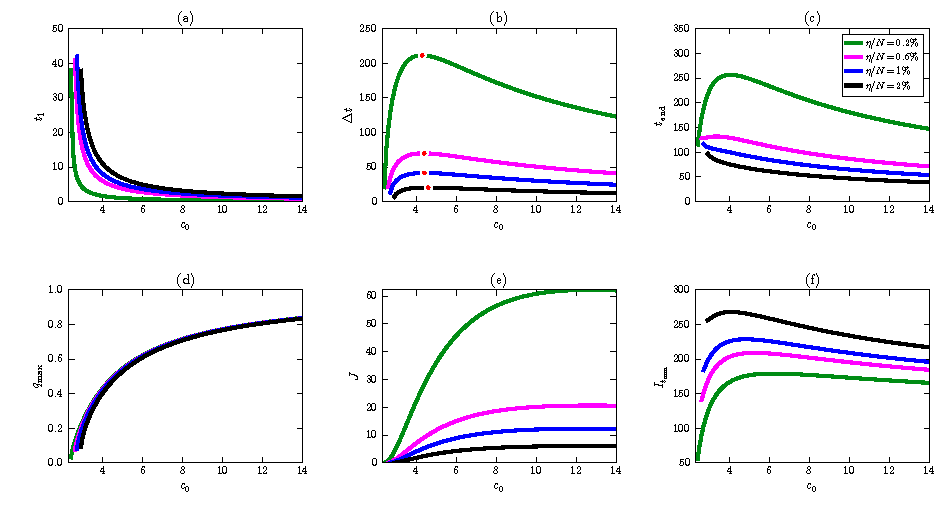
\includegraphics[width=\textwidth]{figures/new4t/S1.pdf}
\caption{基准参数下各指标随常规接触率 $c_0$ 的变化，$\eta/N=0.2\%,0.6\%,1\%,2\%$ 的曲线依次为绿色、品红色、蓝色和黑色，其余参数同正文图~\ref{fig:scenario1:single-sim}；红色圆点为 $\Delta t$ 的数值极大值。(a) 启动时间；(b) 控制时长；(c) 清零时间；(d) 最大隔离比例；(e) 成本 $J$；(f) 总累计新增感染。时间与成本以天计，累计新增感染以人计，$c_0$ 以 $\mathrm d^{-1}$ 计。}
\label{fig:scenario1_summary_c0}
\end{figure}

图~\ref{fig:sup:eta-summary}给出同一组指标随阈值的变化，是正文图~\ref{fig:scenario1_summary_eta}的完整扫描。固定 $c_0$ 时，阈值提高使启动推迟，$q_{\max}$ 只略有下降，控制时长与成本近似与阈值成反比；在所算范围内清零时间缩短，总累计新增感染增加（正文命题~\ref{prop:threshold-tradeoff}）。
\begin{figure}[htbp]
\centering
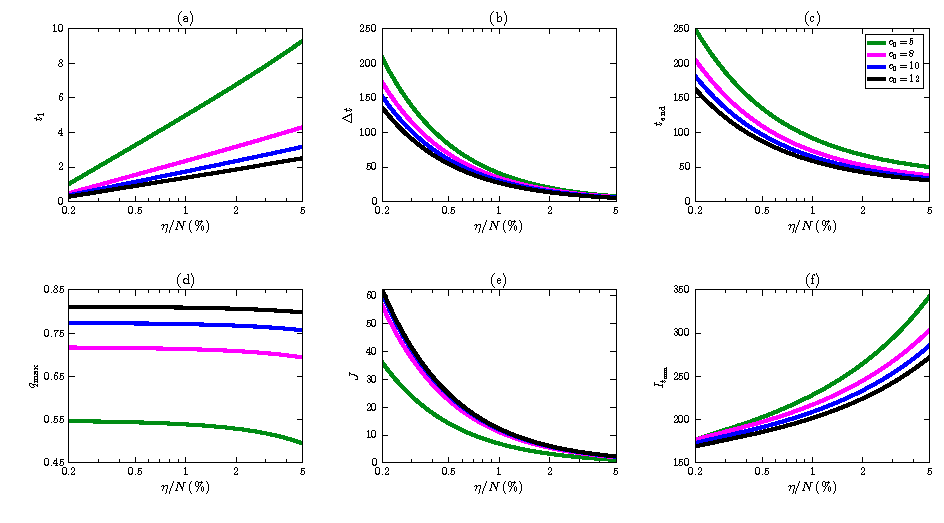
\includegraphics[width=\textwidth]{figures/new4t/S2.pdf}
\caption{基准参数下仅隔离控制的各指标随阈值比例 $\eta/N$ 的变化（横轴为对数刻度），$c_0=5,8,10,12\ \mathrm d^{-1}$ 的曲线依次为绿色、品红色、蓝色和黑色，其余参数同正文图~\ref{fig:scenario1:single-sim}。面板与单位同图~\ref{fig:scenario1_summary_c0}。}
\label{fig:sup:eta-summary}
\end{figure}

图~\ref{fig:baseline:q-joint}给出 $\eta/N=5\%$ 时不同 $c_0$ 与 $c_0=10$ 时不同阈值下的隔离比例轨迹，图~\ref{fig:scenario1_heatmaps_c0_eta}给出 $(\eta/N,c_0)$ 平面上的四项指标。两幅子图中的拐点都在 $\qinf=1-1/[2(1-\beta)]\approx0.4083$ 的同一水平上（正文定理~\ref{thm:s1:inflection}）。$c_0=4$ 时 $q_{\max}=0.3413<\qinf$，即 $S^*<2\bar S$，隔离比例在整个控制期内低于拐点水平，没有内部拐点。

\begin{figure}[htbp]
\centering
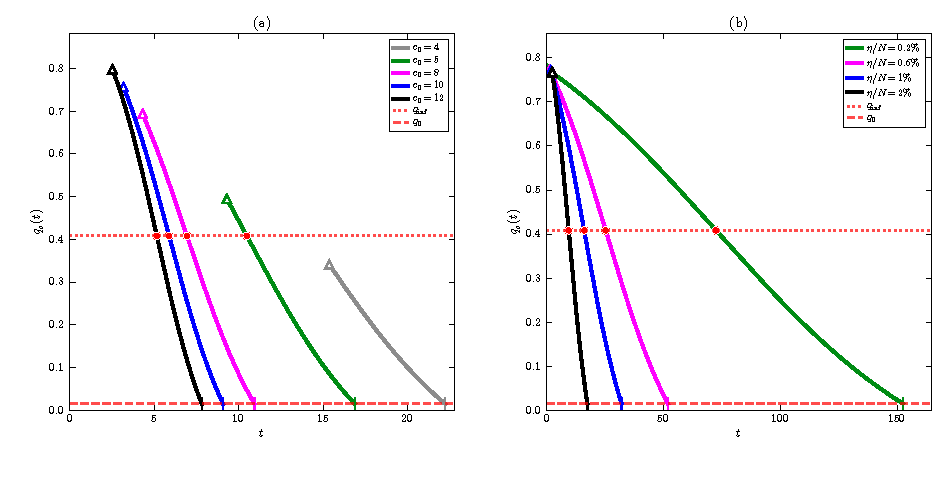
\includegraphics[width=\textwidth]{figures/new4t/S3.pdf}
\caption{不同常规接触率与阈值下仅隔离控制的隔离比例轨迹，其余参数取基准值。(a) $\eta/N=5\%$，$c_0=4,5,8,10,12$ 的曲线依次为灰色、绿色、品红色、蓝色和黑色；(b) $c_0=10$，$\eta/N=0.2\%,0.6\%,1\%,2\%$ 的曲线依次为绿色、品红色、蓝色和黑色。三角形与短竖线分别标出 $t_1$、$t_2$，红点为内部拐点；红色水平虚线为 $q_0$，红色水平点线为 $\qinf\approx0.4083$。}
\label{fig:baseline:q-joint}
\end{figure}

\begin{figure}[htbp]
\centering
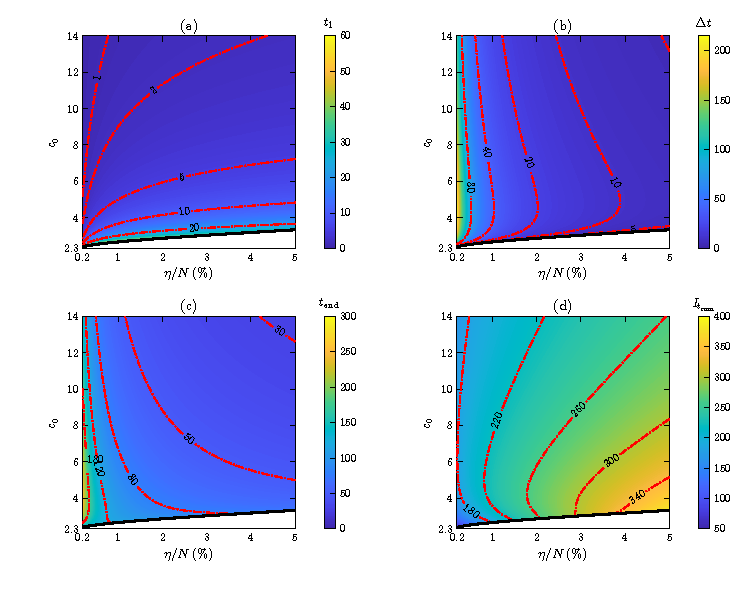
\includegraphics[width=0.8\textwidth]{figures/new4t/S4.pdf}
\caption{$(\eta/N,c_0)$ 平面上仅隔离控制的启动时间、控制时长、清零时间和累计新增感染，其余参数取基准值。黑色实线为触发边界 $c_{0,\min}(\eta)$，白色区域无需加强隔离；红色点划线为等值线，黑色数字为等值。}
\label{fig:scenario1_heatmaps_c0_eta}
\end{figure}

\FloatBarrier
\subsubsection{低阈值极限}
阈值很低时，控制时长与成本按 $1/\theta$ 增长，但这一极限要求初值同时趋于零。固定 $i_0>0$ 时允许的阈值为 $\theta>i_0$，不能在这一问题中直接令 $\theta\to0$。沿同时满足 $i_0\to0$、$\theta\to0$、$0<i_0<\theta$ 的序列，且 $s_0$ 趋于某个大于 $s_c$ 的固定值时，有 $s^*\to s_0$，从而
\begin{equation}
\Delta t\sim\frac1{c_0\theta}\ln\frac{s_0-\bar s}{s_c-\bar s},\qquad
J\sim\frac2{c_0\theta}\int_{s_c}^{s_0}\frac{(1-s_c/s)^2}{s-\bar s}\,ds.
\label{eq:small-threshold}
\end{equation}

相反，固定 $i_0>0$ 而令 $\theta\downarrow i_0$ 时，控制几乎立即启动，控制时长趋于有限值
\[
\frac1{c_0i_0}\ln\frac{s_0-\bar s}{s_c-\bar s}.
\]
因此，由控制时长或成本反解阈值只能在相应的值域内进行，联合小初值极限不能用于固定正初值的问题。

\FloatBarrier
